%-------------------------------------------
\begin{frame}[containsverbatim]
\frametitle{Snakemake point}
%-------------------------------------------
\begin{block}{So far, we've seen:}
\begin{itemize}
    \item the rule and the workflow concepts, the snakefile
    \item how rules are linked thank to input/output files and the first rule, the target rule
    \item how to generalize the inputs of a rule using wildcards on filenames (and the expand function)
    \item how to redirect stdout and sdterr streams (log)
\end{itemize}
\end{block}
\begin{block}{From now, we will seen:}
\begin{itemize}
    \item some snakemake options: to visualize the workflow diagram, use a dry-run option, etc
    \item adding a configuration file
    \item getting file names from the file system
    \item \alert{the container directive ???}
    \item \alert{how to run snakemake on cluster ???}
\end{itemize}
\end{block}
\end{frame}
%-------------------------------------------
\begin{frame}[containsverbatim]
\frametitle{Snakemake DAG visualization}
%-------------------------------------------
\begin{block}{}
Snakemake use Graphviz (\verb|dot| command) to create graphical visualisations, for the complete workflow (--dag) or for the rules dependencies (--rulegraph):
\begin{lstlisting}
snakemake --dag  | dot | display
snakemake --dag  | dot -Tpng > dag.png
\end{lstlisting}
\end{block}
\begin{center}
    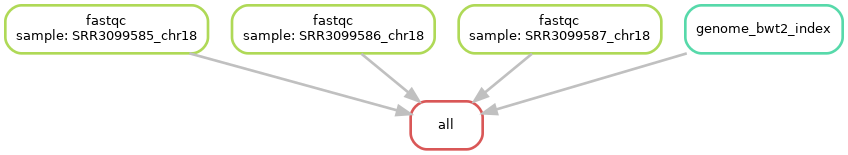
\includegraphics[width=12cm]{03_workflow/images/FAIR_ex1_o7_dag.png}\\
    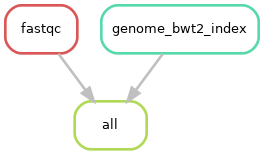
\includegraphics[width=3cm]{03_workflow/images/FAIR_ex1_o5_ruleG.png}
\end{center}
\end{frame}
%-------------------------------------------
\begin{frame}[containsverbatim]
\frametitle{Some Snakemake options}
%-------------------------------------------
\begin{block}{Running options}
\begin{itemize}
    \item automatically create HTML reports (\verb|--report report.html|) containing runtime statistics, a visualization of the workflow topology, used software and data provenance information
    \item dry-run, do not execute anything, display what would be done: \verb|-n --dryrun|
    \item print the executed shell command: \verb|-p --printshellcmds |
    \item print the reason for each rule execution: \verb|-r --reason|
    \item print a summary and status of rule: \verb|-D|
    \item limit the number of jobs in parallel: \verb|-j 1| (cores: \verb|--cores 1|)
\end{itemize}
\end{block}
\vfill
\href{https://snakemake.readthedocs.io/en/stable/executing/cli.html#all-option}{\textcolor{blue}{\underline{all Snakemake options}}}
\end{frame}
%-------------------------------------------
\begin{frame}[containsverbatim]
\frametitle{Some Snakemake options}
%-------------------------------------------
\begin{block}{Configuration file}
Use a configuration file to place all hard-coding values (paths, core numbers, parameters, etc):
\begin{itemize}
    \item can be write both in yml or in json
    \item add Snakemake option: \verb|--configfile file.yml| or add \verb|configfile: file.yml| at the beginning of the snakefile
    \item Snakefile call of defined items: \verb|config["item1"]| in input/output directive and \verb|{config[item1]}| in shell directive
\end{itemize}
\end{block}
\end{frame}
%-------------------------------------------
\begin{frame}[containsverbatim]
\frametitle{File names from the file system}
%-------------------------------------------
To infer the identifiers (IDs) from present files in a directory, use the inbuilt \verb|glob_wildcards| function:
\begin{block}{Ex. of the glob$\_$wilcards function}
\begin{lstlisting}
IDs, = glob_wildcards("thedir/{id}.fastq")
\end{lstlisting}
\end{block}
\verb|glob_wildcards()| matches the given pattern against the files present in the file system and thereby infers the values for all wildcards in the pattern, \verb|{id}| here. 
\vfill
Don't forget the coma after the name (left hand side, \verb|IDs| here).
\end{frame}
%-------------------------------------------
\begin{frame}[containsverbatim]
\frametitle{Conda environment}
%-------------------------------------------
\begin{block}{}
In the practical exercise we will have one conda environment for executing the whole Snakemake workflow. \\
Snakemake also supports using explicit conda environments on a per-rule basis:
\begin{itemize}
    \item add the \verb|conda: rule-specific-env.yml| directive in the rule definition 
    \item run Snakemake with the \verb|--use-conda| option 
\end{itemize}
The specified environment will be created and activated on the fly by Snakemake and the rule will then be run in the conda environment.
\end{block}
\end{frame}
%-------------------------------------------
\begin{frame}[containsverbatim]
\frametitle{Container directive}
%-------------------------------------------
\end{frame}
%-------------------------------------------
\begin{frame}[containsverbatim]
\frametitle{Cluster option}
%-------------------------------------------

\end{frame}
